\section{Materials and Methods}
\subsection{Problem Formulation}
The task of SAR-to-optical translation is formulated as a supervised image-to-image translation problem. Let $\mathcal{X} \subset \mathbb{R}^{H \times W \times C_{in}}$ denote the domain of SAR inputs, where $C_{in}=2$ corresponds to the dual-polarized Sentinel-1 channels (VV, VH) expressed in the decibel (dB) scale. Similarly, let $\mathcal{Y} \subset \mathbb{R}^{H \times W \times C_{out}}$ denote the domain of optical reference images, where $C_{out}=13$ represents the full multispectral stack of Sentinel-2.

The objective is to learn a parametric mapping function $G_{\theta}: \mathcal{X} \rightarrow \mathcal{Y}$, parameterized by $\theta$, such that for a given SAR input $x \in \mathcal{X}$, the generated optical image $\hat{y} = G_{\theta}(x)$ is indistinguishable from the ground truth optical image $y \in \mathcal{Y}$ in terms of spectral and spatial characteristics.

We assume access to a paired dataset $\mathcal{D} = \{(x_i, y_i)\}_{i=1}^{M}$ consisting of spatially co-registered SAR and optical patches acquired over the same geographical regions. The training objective is to find the optimal generator parameters $\theta^*$ that minimize a composite loss function $\mathcal{L}$ over the data distribution:
\begin{equation}
    \theta^* = \arg\min_{\theta} \mathbb{E}_{(x,y) \sim \mathcal{D}} [\mathcal{L}(G_{\theta}(x), y)]
\end{equation}
where $\mathcal{L}$ is a weighted combination of reconstruction, adversarial, and perceptual terms designed to collectively encourage pixel-level accuracy, structural consistency, and spectral fidelity. Specific details on the loss components and optimization strategy are provided in Section~\ref{subsec:losses}.

\subsection{Dataset}
\label{subsec:datasets}

This study utilizes the \textit{SEN12-MS} dataset~\cite{sen12ms_2019}, curated by Schmitt et al. SEN12-MS is a large-scale, globally distributed benchmark explicitly designed to advance research in multimodal Earth observation and deep learning. It comprises 180,662 georeferenced image triplets, each consisting of: (i) dual-polarized Sentinel-1 synthetic aperture radar (SAR) data in VV and VH polarization ($\sigma^{0}$ backscatter values in decibel scale); (ii) full Sentinel-2 multispectral imagery spanning all 13 bands; and (iii) MODIS land cover maps derived from the MCD12Q1 product and resampled to 10 m resolution. Each triplet is stored as a $256 \times 256$ pixel GeoTIFF at 10 m ground sampling distance, corresponding to a spatial coverage of approximately $2.56 \times 2.56$ km per patch. The dataset has a total size of 510 GB, reflecting its high complexity, diversity, and spatial resolution.

The Sentinel-1 component originates from ground-range-detected (GRD) products acquired in interferometric wide swath (IW) mode. The Sentinel-2 imagery was curated using a cloud-free mosaicking workflow on Google Earth Engine, ensuring that each region of interest (ROI) is represented by seasonally consistent, nearly cloud-free multispectral data. Importantly, all triplets underwent manual verification by remote sensing experts to ensure freedom from major artifacts, severe registration errors, or residual cloud contamination.

The ROIs were sampled globally across all inhabited continents and four meteorological seasons of 2017 to maximize spatial and temporal diversity. For the purpose of SAR-to-optical translation, only the Sentinel-1 and Sentinel-2 modalities are utilized; the MODIS component is excluded. Sample data are depicted in Figure~\ref{fig:sen12ms_pairs}.

\begin{figure}[H]
    \centering
    \setlength{\tabcolsep}{1pt} % Minimal horizontal space between images
    \renewcommand{\arraystretch}{0.5} % Minimal vertical space between rows
    
    \begin{tabular}{ccccc}
        % --- Row 1: SAR Images ---
        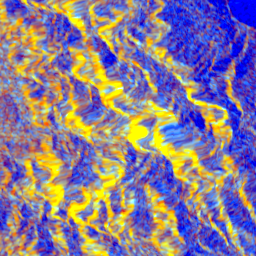
\includegraphics[width=0.19\textwidth]{../latex_source_code/img/ROIs2017_winter_s1_68_p100.png} &
        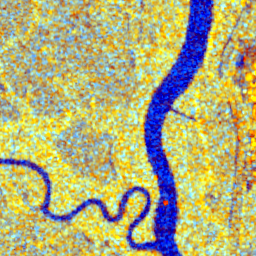
\includegraphics[width=0.19\textwidth]{../latex_source_code/img/ROIs1970_fall_s1_105_p100.png} &
        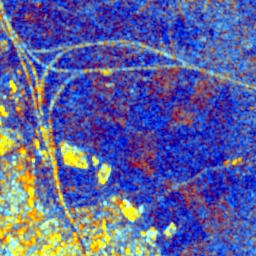
\includegraphics[width=0.19\textwidth]{../latex_source_code/img/ROIs1970_fall_s1_128_p100.png} &
        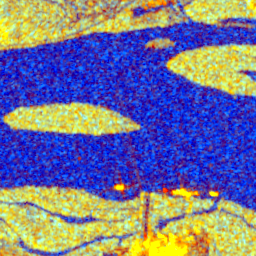
\includegraphics[width=0.19\textwidth]{../latex_source_code/img/ROIs2017_winter_s1_104_p101.png} &
        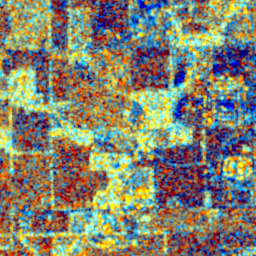
\includegraphics[width=0.19\textwidth]{../latex_source_code/img/ROIs1970_fall_s1_145_p100.png} \\
        
        % --- Row 2: Shared Labels (Middle) ---
        \noalign{\vspace{2pt}} % Tiny gap below SAR images
        \multicolumn{1}{c}{\scriptsize\textit{Winter ROI-68-100}} & 
        \multicolumn{1}{c}{\scriptsize\textit{Fall ROI-105-100}} & 
        \multicolumn{1}{c}{\scriptsize\textit{Fall ROI-128-100}} & 
        \multicolumn{1}{c}{\scriptsize\textit{Winter ROI-104-101}} & 
        \multicolumn{1}{c}{\scriptsize\textit{Fall ROI-145-100}} \\
        \noalign{\vspace{2pt}} % Tiny gap above Optical images
        
        % --- Row 3: Optical Images ---
        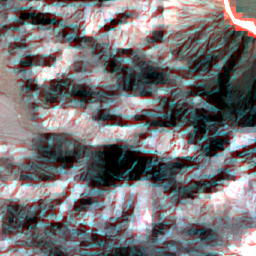
\includegraphics[width=0.19\textwidth]{../latex_source_code/img/ROIs2017_winter_s2_68_p100.png} &
        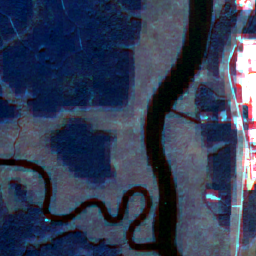
\includegraphics[width=0.19\textwidth]{../latex_source_code/img/ROIs1970_fall_s2_105_p100.png} &
        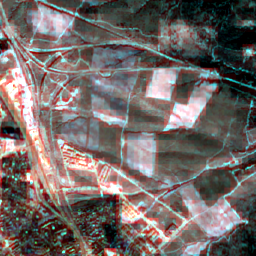
\includegraphics[width=0.19\textwidth]{../latex_source_code/img/ROIs1970_fall_s2_128_p100.png} &
        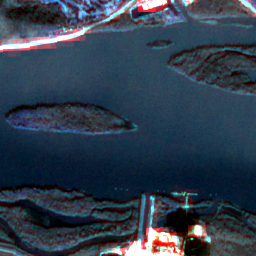
\includegraphics[width=0.19\textwidth]{../latex_source_code/img/ROIs2017_winter_s2_104_p101.png} &
        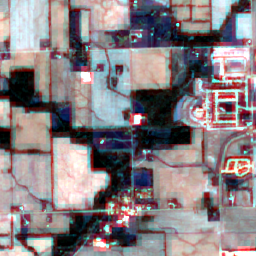
\includegraphics[width=0.19\textwidth]{../latex_source_code/img/ROIs1970_fall_s2_145_p100.png} \\
    \end{tabular}

    \caption{Sample pairs from the SEN12-MS dataset. Top row: Sentinel-1 SAR patches (R: VV, G: VH, B: VV/VH). Middle row: ROI IDs. Bottom row: corresponding Sentinel-2 multispectral patches (RGB visualization).}
    \label{fig:sen12ms_pairs}
\end{figure}

SEN12-MS is part of a broader family of datasets developed to foster multimodal remote sensing research. Its predecessor, SEN1-2~\cite{sen12_2018}, provided SAR–optical pairs but lacked georeferencing, full spectral coverage, and dual-polarization SAR. SEN12-MS addressed these limitations, establishing a comprehensive multimodal benchmark. The family has since been extended by SEN12-MS-CR~\cite{sen12ms-cr_2021} (adding cloudy/cloud-free pairs) and SEN12-MS-CR-TS~\cite{sen12ms-cr-ts_2022} (multimodal time series). This study focuses on SEN12-MS to leverage its global diversity for learning the core SAR-to-optical translation mapping.

\subsubsection{Subset Selection and Preprocessing}
\label{subsec:preprocessing}
The SEN12-MS dataset is divided into four seasonal subsets. Due to the computational demands of extensive experimentation and ablation studies, the \textit{Winter} subset (containing 31,825 paired images) was selected for training and evaluation.

A custom preprocessing pipeline was implemented to standardize the input domains. Following established best practices in the literature~\cite{CR_SEN2_dRNN, c_guided_fus_s2ot, trans_gan_CF, strgb_lat_diff, transfusion_cr}, Sentinel-1 backscatter values were clipped to fixed physical ranges of $[-25, 0]$ dB for VV polarization and $[-32.5, 0]$ dB for VH polarization to suppress radiometric outliers. Similarly, Sentinel-2 top-of-atmosphere (TOA) reflectance values were clipped to the range $[0, 10,000]$. After clipping, all values were linearly normalized to the interval $[-1, 1]$ to align with the Tanh activation function of the generator's output layer. The original spatial resolution of $256 \times 256$ pixels was preserved, and no data augmentation was applied given the inherent global diversity of the dataset.

\subsection{Loss Functions}
\label{subsec:losses}